Neste capítulo iremos descrever alguns métodos da análise topológica de dados
para tratar os diagramas de persistência. 

O primeiro dos métodos é o
gerador ótimo. Para cada ponto no diagrama de persistência, temos um ciclo
associado. A ideia é analisar este ciclo geometricamente e extrair 
informação desse maneira. 
O segundo é a imagem de persistência, um método de vetorização do diagrama de 
persistência, de forma que ele possa ser usado para prever e classificar 
conjuntos de dados. 
Por último, tratamos \textit{mapper}, uma ferramenta da análise topológica 
de dados para visualização de conjuntos de alta dimensão em algum 
espaço de baixa dimensão. 

\section{Geradores ótimos}
O diagrama de persistência nos dá informação sobre buracos e cavidades que
persistentem ao longo de uma filtração. Para cada buraco temos um ciclo
associado, um representante da classe homológica nos grupos de homologia 
da filtração. É possível visualizar esses ciclos através dos simplexos do
complexo simplicial associado a filtração e ao diagrama. Geralmente eles 
podem nos dar informações geométricas, como a localidade de buracos, 
revelando informações escondidas. 

Entretanto, os ciclos por várias vezes não representam de forma ótima
uma propriedade do conjunto. Na Figura~\ref{fig:nonoptcyc} podemos
ver que um ciclo é maior do que poderia ser em relação ao número
de simplexos, não representando de maneira ótima o buraco relacionado. 
\begin{figure}\label{fig:nonoptimal}
    \centering
    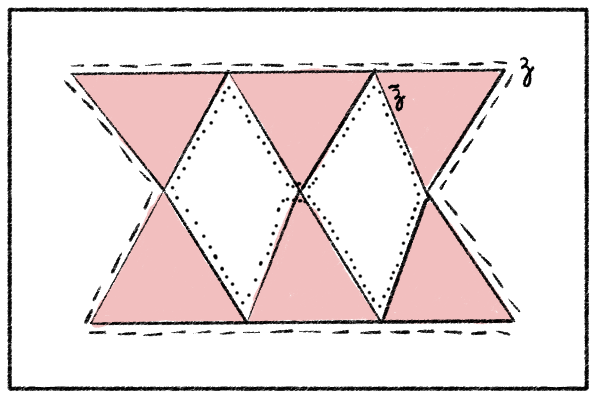
\includegraphics[width=0.7\textwidth]{images/nonoptcyc.png}
    \caption{Dois ciclos homólogos que representam o buraco. Note que o ciclo
            que representa o buraco não é ótimo no número de simplexos. O ciclo
            ótimo é o com linhas pontilhadas.}
    \label{fig:nonoptcyc}
    \fautor
\end{figure} 

A seguir apresentamos a ideia de geradores ótimos, que trata de ajustar
o problema de melhor gerador. Começamos com o problema de otimização
de um único ciclo e depois apresentamos para múltiplos geradores. 
Esta seção tem como referência~\cite{Escolar2015}. 

\subsection{Único Gerador}
Seja $X$ um complexo simplicial qualquer e denote por $Z_q(X)$ o 
conjunto dos $q$-ciclos de $X$, com respeito ao operador bordo $\partial_q$ e 
por denote $B_q(X)$ o conjunto dos $q$-bordos de $X$, em que 
$B_q(X) = \text{im} \partial_{q+1}$.

Para cada $q$, considere $\Set{\sigma_1, \dots, \sigma_N}$ conjunto de $q$-simplexos
de $X$ como a base de $C_q(X)$, grupo de todoas as $q$-cadeias de $X$. Então
representamos todo $x = \sum x_i\sigma_i \in C_q(X)$ por um vetor 
$[x_1, \dots, x_N]^T$. 

Seja agora $z \in Z_q(X)$, considere o problema 
\begin{equation}\label{eq:probfour}
    \begin{split}
        &\text{minimize} \quad \quad ||x||_1 \\
        &\text{sujeito a} \quad \left \{ \begin{array}{l}
            x - \partial_{q+1} y = z \\
            x,y \text{ integrais.}
        \end{array} \right.
    \end{split}
\end{equation}
Aqui tentamos achar um ciclo $\tilde{z}$ homólogo a $z$ que possui 
a menor $1$-norma entre todas as cadeias homólogas a $z$. A $1$-norma é definida
por $\norm{\sum_i x_i\sigma_i}_1 = \sum_i\abs{x_i}$. 

Podemos no entanto alterar o problema. Ao invés de considerar $x$ um vetor inteiro
qualquer, vamos restringir $x$ para valores em $\Set{-1,0,1}$, facilitando a interpretação
geométrica de $\tilde{z}$. Uma consequência disso é $\norm{x}_0 = \norm{x}_1$, em que
$\norm{x}_0 = \abs{\Set{x_i \neq 0}}$ em $C_q(X)$. Adicionamos mais uma condição,
de que para $\tilde{z} = \sum_\sigma n_\sigma \sigma$, $n_\sigma \in \Set{-1,0,1}$. 
Sendo assim, podemos formular o problema anterior da seguinte maneira:

\begin{equation}\label{eq:probfive}
    \begin{split}
        &\text{minimize} \quad \quad ||x||_1 \\
        &\text{sujeito a} \quad \left \{ \begin{array}{l}
            x - \partial_{q+1} y = z \\
            x \text{ é um vetor com entradas em } \Set{-1,0,1} \text{ e } 
            y \text{ é inteiro}
        \end{array} \right.
    \end{split}
\end{equation}

Se $z$ é um vetor com entradas em $\Set{-1,0,1}$, então existe uma solução para o 
problema~\eqref{eq:probfive}~\cite{Dey2010}. Escreva também $x$ como 
$x^+ - x^-$, $\xpos, \xneg \geq 0$ correspondendo as partes positiva e negativa
de $x$ espectivamente. Então podemos reescrever o problema como 

\begin{equation*}
    \begin{split}
        &\text{minimize} \quad \quad ||x||_1 = \sum_{i=1}^N (\xpos_i + \xneg_i) \\
        &\text{sujeito a} \quad \left \{ \begin{array}{l}
            (\xpos - \xneg) - \partial_{q+1} y = z \\
            \xpos, \xneg \text{ com entradas em } \Set{0,1} \text{ e } 
            y \text{ é inteiro,}
        \end{array} \right.
    \end{split}
\end{equation*}
em que $\xpos_i, \xneg_i$ são as entradas dos vetors $\xpos, \xneg$ respectivamente.

A integralidade das soluções não é garantida, precisamos considerar uma
restrição a mais. Uma matrix é dita unimodular se o determinante de cada
submatriz for $-1, 0$ ou $1$. Então podemos garantir uma solução se 
não exigirmos que $\tilde{z}$ seja inteiro e considerar o problema 
de programação linear sobre os reais. Então a unimoludariade total
da matriz de restrição do problema garantirá que o problema possuirá 
solução inteira. Vamos escrever ambos os problemas de seguinte forma:
\begin{equation*}
    \begin{split}
        &\text{minimize} \quad \quad c'x \\
        &\text{sujeito a} \quad \left \{ \begin{array}{l}
            Ax = b \\
            x \geq 0, \text{ inteiro.}
        \end{array} \right.
    \end{split}
\end{equation*}
Para o Problema~\eqref{eq:probfour}, temos
\begin{equation*}
    \begin{split}
        &\text{minimize} \quad \quad  \sum_{i=1}^N (\xpos_i + \xneg_i) \\
        &\text{sujeito a} \quad \left \{ \begin{array}{l}
            \xpos - \xneg - \partial_{q+1}(\ypos - \yneg) = z \\
            \xpos, \xneg, \ypos, \yneg  \geq 0, \text{ inteiros,}
        \end{array} \right.
    \end{split}
\end{equation*}
e possu uma matriz de restrição 
$A = \begin{bmatrix}
I & -I & -\partial_{q+1} & \partial_{q+1}
\end{bmatrix}$. O Problema~\eqref{eq:probfive} também pode ser escrito da forma acima,
bastante colocar a restrição de que $x$ é um vetor com entradas em $\Set{-1,0,1}$ na 
matriz $A$ acima. Então se $\partial{q+1}$ é unimodular, temos que a matriz $A$
também é. 

Para um $q \geq 0$ fixado, existem condições para que $\partial_{q+1}$ seja 
totalmente unimodular~\cite{Dey2010}. Por exemplo, se $X$ é um complexo simplicial finito
triangulando uma variedade compacta de dimensão $q+1$ ou $X$ é um complexo simplicial
finito mergulhado em $\mathbb{R}^{q+1}$, então $\partial_{q+1}$.

\subsection{Múltiplos geradores}
Nem sempre otimizar apenas um gerador é suficiente. Como podemos ver na Figura~\ref{fig:nonoptimal},
os dois ciclos não são os ótimos, mesmo após o processo de otimização. Podemos dizer intuitivamente
que o ciclo está emperrado entre os dois buracos. Vamos modificar a proposta e resolver este problema. 

Seja $\Set{g_1, \dots, g_m}$ um conjunto de ciclos. Considere agora o seguinte problema
\begin{equation*}
    \begin{split}
        &\text{minimize} \quad \norm{x}_1 \\
        &\text{sujeito a} \quad \left \{ \begin{array}{l}
            x- \partial_{q+1}(y) + \sum_{j=1}^m a_j g_j = z \\
            x, y \text{ e } a \text{ inteiros,}
        \end{array} \right.
    \end{split}
\end{equation*}
e seja $P(z;g_1, \dots, g_m)$ o conjutno de soluções ótimos projetado na variável
$x$ do problema acima. Linearizando o problema, obtemos
 \begin{equation*}
    \begin{split}
        &\text{minimize} \quad \quad  \sum_{i=1}^N (\xpos_i + \xneg_i) \\
        &\text{sujeito a} \quad \left \{ \begin{array}{l}
            \xpos - \xneg - \partial_{q+1}(y) + \sum_{j=1}^m a_j g_j = z \\
            \xpos, \xneg \geq 0, \xpos, \xneg, y, \text{ e } a \text{ inteiros.}
        \end{array} \right.
    \end{split}
\end{equation*}

Vamos agora entender os ciclos $g_1, \dots, g_m$. Estes são os ciclos que 
gostariamos de tirar enquanto otimizando o ciclo $z$, em outras palavras,
preencheriamos os buracos que ficam entre $z$ e o seu ciclo ótimo,
onde esses buracos são representados por $g_i$, para todo $i$. Estes ciclos
são chamados de ciclos relativos e a soma $\sum a_j g_j$ pode ser entedida
da seguinte forma. Seja 
\begin{equation*}
    \partial^{'}_{q+1} = \begin{bmatrix} \partial_{q+1} & g_1 & \dots & g_m \end{bmatrix}
\end{equation*}
a matriz de bordo com colunas a mais, $g_1, \dots, g_m$. Geometricamente, estamos
adicionando células $\tau_j$ em $X_{q+1}$ de forma que $\partial^{'}_{q+1} \tau_j 
= g_j$ para $j=1,\dots,m$. Como dito anteriormente, cada célula $\tau_j$ cobre
uma propriedade topológica, permitindo que $z$ passe por $g_j$. 

Seja agora $\Set{z_1, \dots, z_n}$ conjunto gerador de $H_q(X)$, grupo de homologia
de $X$. Portanto, se trocarmos $z_j$ por algum
\begin{equation*}
    \tilde{z}_j \in P(z_j; z_1, \dots, z_{j-1}, z_{j+1}, \dots, z_n),
\end{equation*}
temos que $\Set{z_1, \dots, \tilde{z}_j, \dots, z_n}$ é um novo conjunto gerador 
de $H_q(X)$, já que 
\begin{equation*}
    [\tilde{z}_j] = [z_j] + \sum_{i\neq j} a_i [z_i],
\end{equation*}
pelas restrições do problema de otimização. Portanto, temos o Algoritmo~\ref{alg:optimize_cycles}.
\begin{algoritmo}[!htpb]
  \caption{Procedimento de otimização dos geradores.}
  \label{alg:optimize_cycles}
  \begin{algorithmic}[1]
    \Require Geradores $z_1, \dots, z_m$ de $H_q(X)$
    \Function{optimize\_cycles}{$\Set{z_1, \dots, z_n}$}
    \For{$j \in \Set{1,\dots,n}$}
        \State Escolha $\tilde{z}_j$ de $P(z_j; \tilde{z}_1, \dots,
         \tilde{z}_{j-1}, z_{j+1}, \dots, z_n)$
    \EndFor    
    \State \Return $\Set{\tilde{z}_1, \dots, \tilde{z}_n}$
    \EndFunction
  \end{algorithmic}
\end{algoritmo}


\subsection{Geradores ótimos em homologia persistente}

Seja $\emptyset = X_0 \subset X_1 \subset \dots \subset X_N$ uma filtração com a propriedade de que 
em cada índice, apenas um simplexo é adicionado, ou seja, se $\sigma_j$ é um simplexo, então
$X_j \backslash X_{j-1} = \sigma_j$, dessa forma cada simplexo causa o nascimento ou morte de uma 
classe de homologia. Também para cada simplexo em $X_N$, temos um índice $j$ de nascimento único. 

Vamos agora descrever os passos para otimizar os ciclos gerados utilizando o algoritmo de persistência.
Denote por $A_j$ o bordo do simplexo $\sigma_j$, $A_j = \partial \sigma_j$. O bordo do simplexo é
representado como um vetor na base de todos os simplexos de $X$, ordenados de acordo com o índice da
filtração. A i-ésima entrada de $A_j$ é denotada por $A_j(i)$. Para qualquer coluna
$A_j$, o seu pivot é denotado por $\pivot(A_j)$ representa o maior inteiro $i$ tal que 
$A_j(i) \neq 0$.

O Algoritmo~\ref{alg:redhir} calcula a persistência da filtração $X$. Note que neste caso específico
utilizamos coeficientes em $\mathbb{Q}$. 

\begin{algoritmo}[htpb!]
    \caption{Algoritmo para calcular o diagrama de persistência de uma filtração.}
    \label{alg:redhir}
    \begin{algorithmic}[1]
        \Procedure{compute\_persistence}{X}
            \State Inicialize $g_j = \sigma_j$ para todo $j=1,\dots,N$.
            \For{$j=1,\dots,N$}
                \While{$A_j \neq 0$ e $l(\pivot(A_j)) \neq 0$}
                    \State $p \leftarrow \pivot(A_j)$
                    \State $r \leftarrow -\frac{A_j(p)}{A_{l(p)}(p)}$
                    \State $A_j \leftarrow + r \cdot A_{l(p)}$
                    \State $g_j \leftarrow + r \cdot g_{l(p)}$
                \EndWhile
                \If{$A_j \neq 0$} 
                    \State $i \leftarrow \pivot(A_j)$
                    \State $l(i) \leftarrow j$ 
                    \State Insira o par $(i,j)$ na matriz dgm
                \EndIf
            \EndFor
            \ForAll{$i$ tal que $i\neq b,d$ para todo $(b,d) \in \text{dgm}$}
                \State Insira $(i, \infty)$ em dgm. 
            \EndFor
            \State \Return dgm     
        \EndProcedure 
    \end{algorithmic}
\end{algoritmo}

Para cada $p$, o valor $l(p)$ registra na tabela $l$ o índice da coluna reduzida que possui o pivot na linha $p$.  
Temos então dois casos, se $A_j$ é reduzida a uma coluna nula, então temos o nascimento de um ciclo $g_j$. 
Caso contrário, temos a morte de um ciclo que nasceu em $i = \pivot(A_j)$. Além disso, a mudança na base é 
atualizada e salva nos ciclos $g_j$. No final do algoritmo todo índice $i$ é pareado com algum índice $j$ ou 
não é. Sendo assim, denote por 
\begin{equation*}
    d(i) = \left\{
    \begin{array}{cl}
        j      & \text{ se } (i,j) \text{ é o par de } i, \\
        \infty & \text{ se } i \text{ não é pareado}, 
    \end{array}
    \right.
\end{equation*}
o índice de morte do ciclo que nasce no tempo $i$. Defina então
\begin{equation*}
    \mathcal{L}_q(k) = \Set{i | i \leq k, A_i = 0, \dim\sigma_i = q, d(i) > k}.
\end{equation*}
O conjunto de índices acima representa todos os ciclos que nascem antes de $\sigma_k$ e 
não se tornam parte do borde de $X_k$. Pode-se mostrar que 
\begin{equation*}
    \Set{[g_i] | i \in \mathcal{L}_q(k)}
\end{equation*}
forma uma base de $H_q(X_k)$. 

Com a dimensão $q$ fixada, o Algoritmo~\ref{alg:optcycles} calcula os ciclos ótimos logo após 
o seu nascimento. 

\begin{algoritmo}[htpb!]
    \caption{Algoritmo para calcular o diagrama de persistência de uma filtração e os ciclos ótimos.}
    \label{alg:optcycles}
    \begin{algorithmic}[1]
        \Procedure{persistence\_optimal\_cycles}{X,q}
            \State Inicialize uma tabela $l$
            \State $B$, uma matriz vazia
            \State Inicialize $g_j = \sigma_j$ para todo $j=1,\dots,N$.
            \For{$j=1,\dots,N$}
                \If{$\dim\sigma_j = q$}
                    \State Atualize o problema de otimização com o novo simplexo $\sigma_j$
                \EndIf
                \While{$A_j \neq 0$ e $l(\pivot(A_j)) \neq 0$}
                    \State $p \leftarrow \pivot(A_j)$
                    \State $r \leftarrow -\frac{A_j(p)}{A_{l(p)}(p)}$
                    \State $A_j \leftarrow + r \cdot A_{l(p)}$
                    \State $g_j \leftarrow + r \cdot g_{l(p)}$
                \EndWhile
                \If{$A_j=0$ e $\dim\sigma_j=0$}
                    \State $\tilde{z}_j = \textsc{optimize\_cycle}(g_j)$
                    \State Atualize o problema de otimização com $\tilde{z}_j$
                \EndIf
                \If{$A_j \neq 0$} 
                    \State $i \leftarrow \pivot(A_j)$
                    \State $l(i) \leftarrow j$ 
                    \State Insira o par $(i,j)$ na matriz dgm
                    \If{$\dim\sigma_j = q + 1$}
                        \State Adicione $A_j$ a matrix $B$ (como uma coluna de bordo)
                        \State Remova $\tilde{z}_i$ do problema de otimização
                    \EndIf
                \EndIf
            \EndFor
            \ForAll{$i$ tal que $i\neq b,d$ para todo $(b,d) \in \text{dgm}$}
                \State Insira $(i, \infty)$ em dgm. 
            \EndFor
            \State \Return dgm     
        \EndProcedure 
    \end{algorithmic}
\end{algoritmo}

Quando um simplexo $\sigma_j$ de dimensão $q$ é encontrado, atualizamos o problema de timização
com uma nova variável e uma restrição correspondendo ao seu ciclo. No Problema~\eqref{eq:optimize}
a variável $x$ aumenta em um no seu tamanho e as restrições são completadas com zeros.

\begin{algoritmo}
    \caption{Procedimento para encontrar o ciclo ótimo.}
    \label{alg:optimize}
    \begin{algorithmic}[1]
        \Procedure{optimize\_cycle}{$z_j = g_j$}
            \State Encontre uma solução ótima $\tilde{z}_j$ para
            \begin{equation}\label{eq:optimize}
                \begin{array}{rl}
                    \text{minimize } & \norm{x}_1 \\
                    \text{sujeito a } & 
                    \left\{x + By + \mathlarger{\sum}_{i \in \mathcal{L}_q(j), i < j} a_i \tilde{z}_i = z_j\right.
                \end{array}
            \end{equation}
            \State \Return $\tilde{z}_j$
        \EndProcedure
    \end{algorithmic}
\end{algoritmo}

Se a coluna $A_j$ é zerada, isso significa o nascimento de um novo ciclo. Se sua dimensão for
$q$, então resolvemos o problema de otimização com o ciclo $g_j = z_j$ que acabou de nascer. 
Uma vez com o ciclo otimizado $\ztilde_j$, o adicionamos no problema de otimização como um
ciclo relativo. 

Se a coluna $A_j$ não for zerada, isso sinaliza a morte de um ciclo e se $\dim \sigma_j = q + 1$,
então adicionamos a coluna $A_j$ no problema de otimização como uma coluna no final da matriz de bordo $B$.
Além disso, se $low(j) = i$, isso significa que o ciclo $\ztilde_i$ de dimensão $q$ faz parte do bordo. 
Portanto, o ciclo $\ztilde_i$ não é mais necessário no processo de otimização, e assim o removemos
do problema. 

No Teorema~\ref{teo:optimize_cycle} mostramos que os ciclos otimizados forma uma base para cada 
grupo de homologia na filtração de $X$, mantendo a consistência da informação topológica dada
pelo diagrama de persistência. 
\begin{teo}\label{teo:optimize_cycle}
    Seja $q$ um número inteiro não negativo. Sejam então $\tilde{z}_1, \dots, \tilde{z}_m$ os 
    ciclos ótimos gerados pelo Algoritmo~\ref{alg:optcycles}. Então 
    $\Set{[\tilde{z}_i] | i \in \mathcal{L}_q(k)}$ forma uma base de $H_q(X)$.
\end{teo}
\begin{proof}
    A classe $[\ztilde_i] \in H_q(X_k)$ satisfaz, 
    \begin{equation*}
        [\ztilde_i] = [g_i] + \sum_{h\in \mathcal{L}_q(i), h<i} a_h[\ztilde_h]
    \end{equation*}
    pelo Problema~\ref{eq:optimize} e pelo fato de que $B = \text{img}\left.
    \partial_{q+1}\right|_{X_k}$. De maneira similar para $[\ztilde_h]$, 
    \begin{equation}\label{eq:ztilde}
        [\ztilde_i] = [g_i] + \sum_{h<i, A_h = 0, \dim\sigma_h = q} c_h [g_h]. 
    \end{equation}
    O subíndice da soma em~\eqref{eq:ztilde} se refere a todos os ciclos que nascem antes
    de $i$ e possuem dimensão $q$. Agora queremos os índices $h$ tais que $d(h) > k$, de 
    forma que obtemos a soma
    \begin{equation}\label{eq:basisopt}
        [\ztilde_i] = [g_i] + \sum_{h \in \mathcal{L}_q(k), h<i}.
    \end{equation}  
    
    Quando expandimos cada $[\ztilde_h] = [g_h] + \sum_{h' \in \mathcal{L}_q(k)} 
    a'_{h'}[\ztilde'_{h'}$, não sabemos se para $h'$ e seus ciclos correspondentes
    $g_{h'}$ vivem até o índice $k$. Para aqueles $h'$ com $d(h') \leq k, [g_{h'}]$,
    já que eles morrem antes ou quando entram em $H_q(X_k)$. Então, para os índices $h$
    que satisfazem essa propriedade, $[g_h]$ entra no bordo e podemos remove-los da soma
    em~\eqref{eq:ztilde}. Logo, obtemos~\eqref{eq:basisopt}. 

    Agora, a transformação induzida por~\eqref{eq:basisopt} é invertível, pois a condição
    $h < i$ implica que a matriz de tranformação é triangula com $1$'s na diagonal. 
\end{proof} 

A implementação deste método foi feita pelos autores do artigo original~\cite{Escolar2015} e
pode ser encontrada no site: \url{https://bitbucket.org/remere/optiperslp}.
\section{Vetorização do diagrama de persistência}
Dado uma sequência de conjuntos de dados $X_i$ e os respectivos diagramas de persistência tem-se uma variação no
seus tamanhos, devido a natureza do algoritmo de homologia persistente. Além de variação entre os tamanhos, cada 
diagrama é um multi-conjunto, sendo mais difícil de analisar-los. Ao utilizar algoritmos de machine learning, 
assume-se entradas com tamanhos fixos no conjunto inteiro de dados. Portanto diagramas de persistências descrevendo
uma sequência de proteínas, por exemplo, precisam ser vetorizados de alguma forma antes de podermos utilizar em
conjunto com outros algoritmos, como redes neurais ou regressão linear. 

Existem várias formas de vetorização de um diagrama de persistência, como \textit{Persistence landscapes}
\cite{bubenik15a} e Imagem de persistência (\textit{Persistence Image}) \cite{Adams2017}. Neste trabalho apresentamos
a imagem de persistência e alguns exemplos.

\subsection{Estabilidade da Imagem de Persistência}
Imagem de persistência é uma vetorização de forma que o respectivo diagrama é representado como 
uma imagem de tamanho fixo $(n,m)$. De forma intuitiva esse método é uma forma de suavização do diagrama 
de persistência, em que uma gaussiana é centrada em cada ponto e depois são somadas com peso. Abaixo descrevemos
formalmente o processo para obter uma imagem de persistência.

Seja $D = \Set{(b_i,d_i)}_{i}$ um diagrama de persistência em alguma dimensão e considere $T(x,y) = (x, y-x)$ 
uma transformação linear em $\mathbb{R}^2$. Seja $T(B)$ o multiconjunto decorrente da transformação linear $T$
aplicada em $B$ onde cada ponto $(x,y) \in B$ corresponde ao ponto $(x,y-x) \in T(B)$. Considere agora uma 
função de probabilidade diferenciável $\phi_u\colon \mathbb{R}^2 \to \mathbb{R}$ com média $u=(u_x, u_y)$. 

Fixe agora uma função peso $f\colon \mathbb{R}^2 \to \mathbb{R}$ de tal forma que ela é zero no eixo horizontal,
contínua e diferenciável por partes. É importante que essas condições sejam satisfeitas, pois elas garante
a estabilidade da imagem de persistência sob a distância $1$-Wasserstein. Dessa forma temos a seguinte definição. 

\begin{defi}
    Para um diagrama de persistência $B$, a correspondente superfície de persistência $\rho_B \colon \mathbb{R}^2
    \to \mathbb{R}$ é a função dada por 
    \begin{equation*}
        \rho_B(z) = \sum_{u \in T(B)} f(u) \phi_u(z). 
    \end{equation*}
\end{defi}

Entretanto, um computador não consegue utilizar uma função para fazer cálculos e estimativas, ela precisa
ser vetorizada (ou discretizada) de alguma forma. Desta forma, vamos discretizar $\rho_B$ em um domínio específico,
que depende de $T(B)$. Em específico, fixamos um grid e o valor de cada pixel é dado pela integral nessa região.

\begin{defi}
    Seja B um diagrama de persistência. A imagem de persistência de B é a coleção de pixeis 
    \begin{equation*}
        I(\rho_B)_p = \iint_p \rho_B dydx.
    \end{equation*}
\end{defi}

Na vetorização do diagrama alguns parâmetros precisam ser estabelecidos. Em \cite{Adams2017} mostra-se que
as imagens são robustas sob a escolha da resolução (tamanho do grid). A outra escolha é a distribuição e dependendo
a variância. Em \cite{Adams2017} a distribuição gaussiana é utilizada com variância dependendo do problema e 
sendo assim o usuário a escolhe. Por último, a escolha da função peso, que pode variar de problema pra problema.
A função abaixo é um exemplo utilizado por \cite{Adams2017}. Observe que para pontos com valores altos de 
persistência tem um valor maior também. Mas com problemas que pontos de baixa ou média persistência são importantes,
a utilização de outros pontos se faz necessária. 

\begin{equation}\label{eq:weightfunct}
    w_b(t) = \left\{
             \begin{array}{@{}ll@{}} 
                 0           & \text{ if } t \leq 0, \\
                 \frac{t}{b} & \text{ if } 0 < t < b, \\
                 1           & \text{ if } t \geq b, 
             \end{array}\right.
\end{equation}
onde $b$ é considerado o valor de maior persistência em $T(B)$.

Em vários conjuntos é normal que apresentem ruídos e algumas variações, assim dando diagramas de persistência
diferentes. Entretanto, há uma medida para avaliar a distância entre eles. 
\begin{defi}
    A distância $p$-Wasserstein definida entre dois diagramas de persistência B e B' é dada por 
    \begin{equation*}
        W_p(B,B') = \inf_{\gamma\colon B \to B'} \left( \sum_{u\in B} \norm{u - \gamma(u)}_{\infty}^{p} 
                    \right)^\frac{1}{p},
    \end{equation*}
    onde $1 \leq p < \infty$ e $\gamma$ é bijeção entre $B$ e $B'$. 
\end{defi}

Seja $h\colon \mathbb{R}^2 \to \mathbb{R}$ uma função diferenciável. Denote 
$\mid \nabla h \mid = \sup_{z\in \mathbb{R}^2} \norm{\nabla h(z)}_2$. Pelo teorema do valor médio, temos que 
\begin{equation}\label{eq:mean_val}
    \mid h(u) - h(v) \mid \leq \mid \nabla h \mid \norm{u-v}_2.
\end{equation}

Seja $u,v\in \mathbb{R}^2$ e considere as duas distribuições diferenciáveis $\phi_u, \phi_v$. Como o supremo e 
a derivada de direção maximal de uma distribuição de probabilidade diferenciável são invariantes por translação,
podemos denotar $\mid \nabla \phi_u \mid$ por $\mid \nabla \phi \mid$ e $\norm{\phi_u}_\infty$ por
$\norm{\phi}_\infty$. E observe ainda devido a invariância pela translação, temos que 
\begin{equation}\label{eq:mean_val_dist}
    \norm{\phi_u - \phi_v}_\infty \leq \mid \nabla \phi \mid \norm{u-v}_2.
\end{equation} 

Vamos enunciar um lema agora que será utilizado nas provas de estabilidade das imagens de superfície e persistência.

\begin{lem}\label{lema:persimg}
    Sejam $u,v\in \mathbb{R}^2$, então $\norm{f(u)\phi_u - f(v)\phi_v} \leq 
    \left( \norm{f}_\infty \mid \nabla \phi \mid + \norm{\phi}_\infty \mid \nabla f \mid \right) \norm{u-v}_2.$
\end{lem}
\begin{demonstracao}
Seja $z\in \mathbb{R}^2$ qualquer, então
\begin{align*}
  \begin{split}
    \abs{f(u)\phi_u(z) - f(v)\phi_v(z)} &= \abs{f(u) \left(\phi_u(z) - \phi_v(z)\right) + \left( f(u) - f(v)\right)
    \phi_v(z)} \\
    &\leq \norm{f}_\infty \abs{\phi_u(z) - \phi_v(z)} + \norm{\phi}_\infty \abs{f(u) - f(v)}\\
    &\leq \norm{f}_\infty \abs{\nabla \phi} \norm{u-v}_2 + \norm{\phi}_\infty + \abs{\nabla f} \norm{u-v}_2 
     \quad \text{por \ref{eq:mean_val_dist} e \ref{eq:mean_val}}\\
    &= \left( \norm{f}_\infty \abs{\nabla \phi} + \norm{\phi}_\infty + \abs{\nabla f}\right) \norm{u-v}_2.
  \end{split}
\end{align*}
\end{demonstracao}

\begin{teo}\label{teo:surf_stab}
  A superfície de persistência é estável em relação a distância $1$-Wasserstein. Dados $B,B'$ diagramas de 
  persistência finitos, temos que 
  \begin{equation*}
    \norm{\rho_B - \rho_{B'}}_\infty \leq \sqrt{10} 
    \left( \norm{f}_\infty \abs{\nabla \phi} + \norm{\phi}_\infty + \abs{\nabla f}\right) W_1(B,B')
  \end{equation*}
\end{teo}
\begin{demonstracao}
  Por hipótese, B e B' são finitos, logo existe uma bijeção entre $B$ e $B'$ que atinge o ínfimo da distância 
  de Wasserstein. Portanto
  \begin{align*}
  \begin{array}{lll}
    \norm{\rho_B - \rho_{B'}}_\infty &= 
                \norm{\sum_{u\in T(B)}f(u)\phi_u - \sum_{u\in T(B)}f(\gamma(u))\phi_{\gamma(u)}}_\infty \\
    &\leq \sum_{u\in T(B)} \norm{f(u)\phi_u - f(\gamma(u))\phi_{\gamma(u)}} & \\
    &\leq \left( \norm{f}_\infty \abs{\nabla \phi} + \norm{\phi}_\infty + \abs{\nabla f}\right) 
            \sum_{u\in T(B)} \norm{u-\gamma(u)}_2 &  \text{por \ref{lema:persimg}}\\
    &\leq \sqrt{2} \left( \norm{f}_\infty \abs{\nabla \phi} + \norm{\phi}_\infty + \abs{\nabla f}\right) 
            \sum_{u\in T(B)} \norm{u-\gamma(u)}_\infty & \text{já que } \norm{\cdot}_2 \leq \sqrt{2} 
            \norm{\cdot}_\infty \text{ em } \mathbb{R}^2 \\
    &\leq \sqrt{10} \left( \norm{f}_\infty \abs{\nabla \phi} + \norm{\phi}_\infty + \abs{\nabla f}\right) 
             \sum_{u\in T(B)} \norm{u-\gamma(u)}_\infty & \text{já que } \norm{T(\cdot)}_2 
             \leq \sqrt{5}\norm{\cdot}_\infty\\
    &=\sqrt{10} \left( \norm{f}_\infty \abs{\nabla \phi} + \norm{\phi}_\infty + \abs{\nabla f}\right) W_1(B,B'). &
  \end{array}
  \end{align*}
A última desigualdade é necessária, pois a distância de Wasserstein é definida sobre os pontos do diagrama de 
persistência que são da forma nascimento e morte, não nascimento e persistência. 
\end{demonstracao}

E por fim, temos que as imagens de persistência são estáveis.
\begin{teo}
    A imagem de persistência é estável em relaçaõ a distância $1$-Wasserstein. Se $A$ é o valor máximo dentre 
    todos os pixeis da imagem, então 
    \begin{equation}
        \norm{I(\rho_B) - I(\rho_{B'})}_\infty \leq 
        \sqrt{10} \left( \norm{f}_\infty \abs{\nabla \phi} + \norm{\phi}_\infty + \abs{\nabla f}\right) W_1(B,B').
    \end{equation}
\end{teo}
\begin{demonstracao}
  A demonstração segue do Teorema \ref{teo:surf_stab} e do fato que para um pixel $p$ qualquer 
  \begin{equation*}
    \abs{I(\rho_B)_p - I(\rho_{B'})_p} \leq A(p) \norm{\rho_B - \rho_{B'}}_\infty,
  \end{equation*}
  em que $A(p)$ representa a área do píxel $p$. 
\end{demonstracao}

\subsection{Exemplos de Imagens de Persistência}
Considere $X$ um conjunto de pontos extraídos de um círculo com ruído, como pode ser visto na 
\autoref{fig:noisycircle}.
\begin{figure}[!htbp]
    \centering
    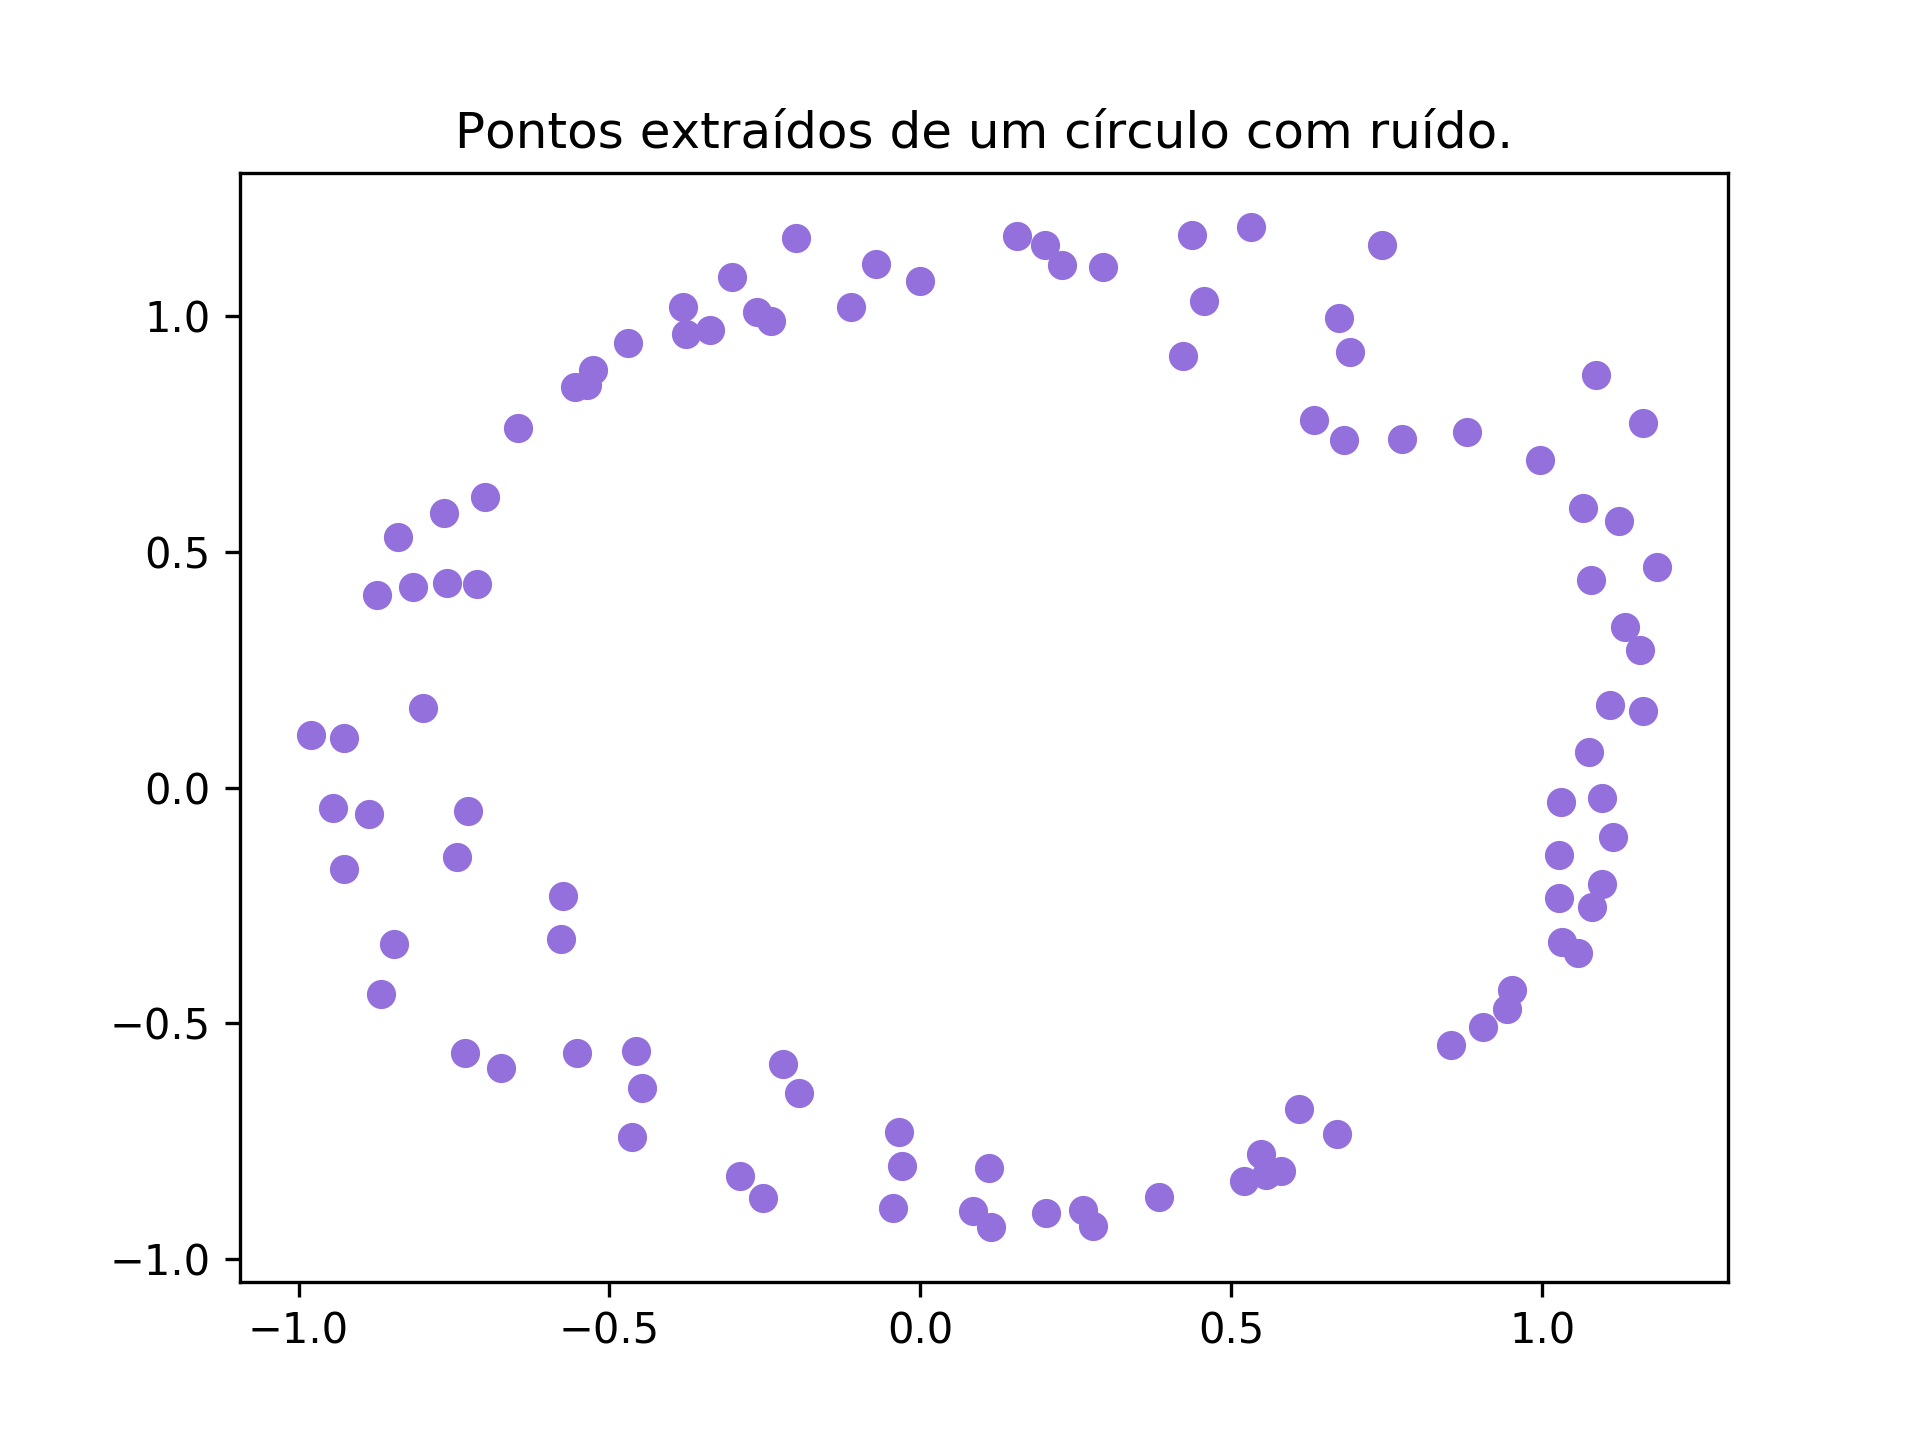
\includegraphics[width=0.7\textwidth]{images/noisy_circle.png}
    \caption{Pontos extraídos de um círculo com ruídos.}
    \label{fig:noisycircle}
    \fautor
\end{figure}
Na \autoref{fig:persdcircle} tem-se os diagramas de persistência do círculo de dimensão $0$ e $1$, assim mostrando
as componentes conexas e buracos. Note que existem dois pontos longe da diagonal, um representando a 
componente conexa e o outro o buraco do círculo.  
\begin{figure}[!htbp]
    \centering
    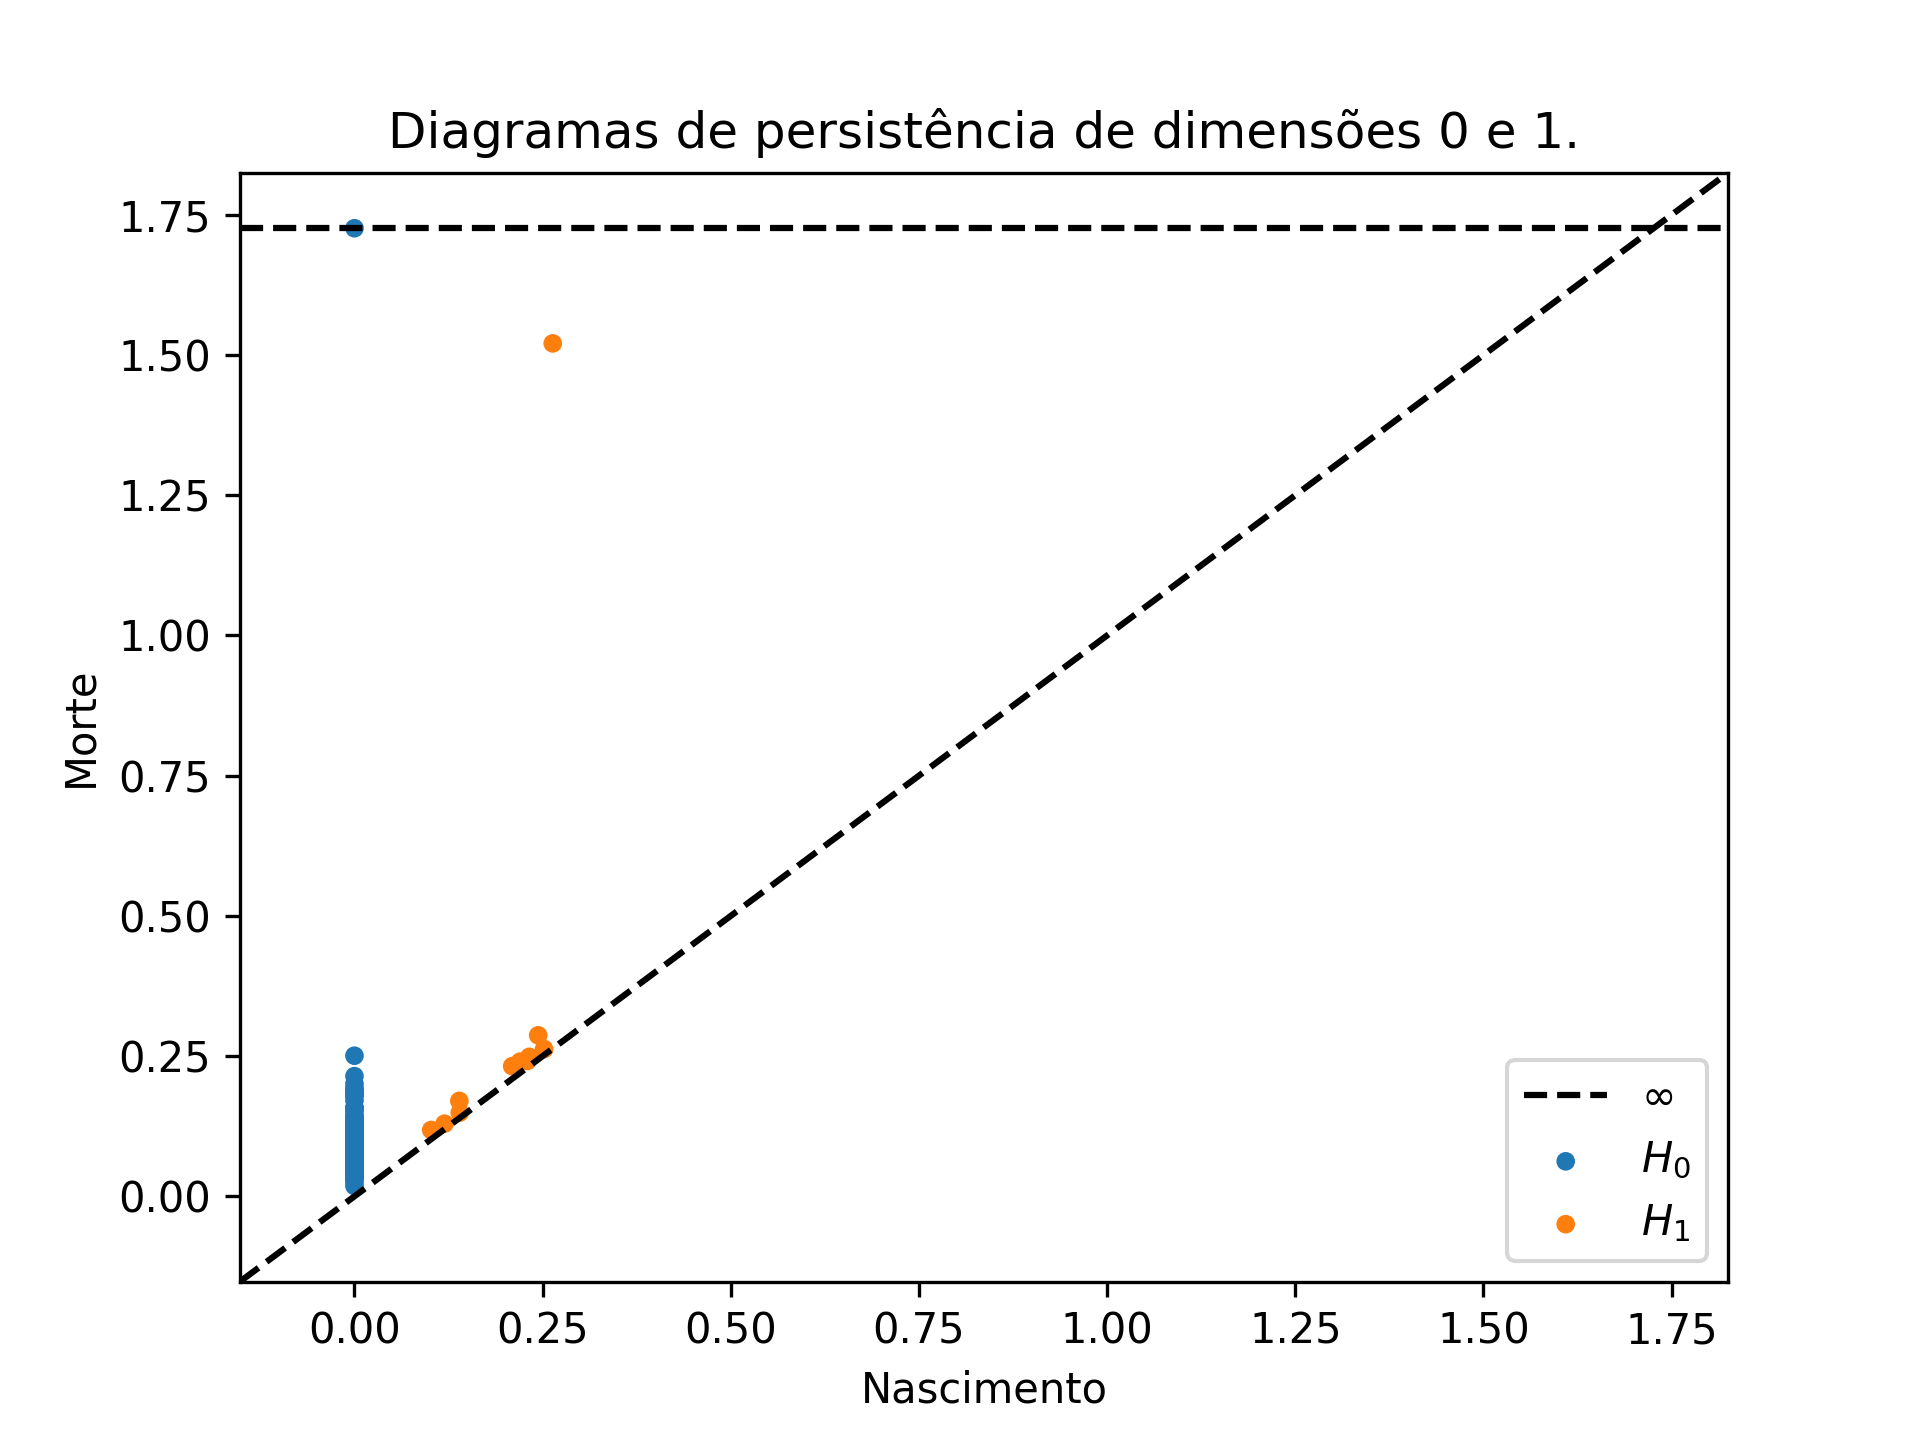
\includegraphics[width=0.7\textwidth]{images/persdcircle.png}
    \caption{Diagrams de persistência do círculo $X$. Em laranja o diagrama de persistência de dimensão $1$,  
            em azul o de dimensão $0$. A filtração de Vietoris-Rips foi usada para calcular o complexo simplicial.}
    \label{fig:persdcircle}
    \fautor
\end{figure}
Vamos agora análisar as imagens de persistência para cada uma das images. Escolhemos a distribuição gaussiana
dada por 
\begin{equation*}
    g_u(x,y) = \frac{1}{2\pi\sigma^2}e^{-((x-u_x)^2 + (y-u_y)^2)/2\sigma^2}.
\end{equation*}
A \autoref{eq:weightfunct} é utilizada como função peso. Para calcular as imagens de persistência 
definimos três variâncias: $0.001, 0.1, 1.0$, e dois tamanhos de imagem: 
$10\times10$ e $50\times50$. O resultado pode ser visto na \autoref{fig:persimgcircle}.
\begin{figure}[!htbp]
    \centering
    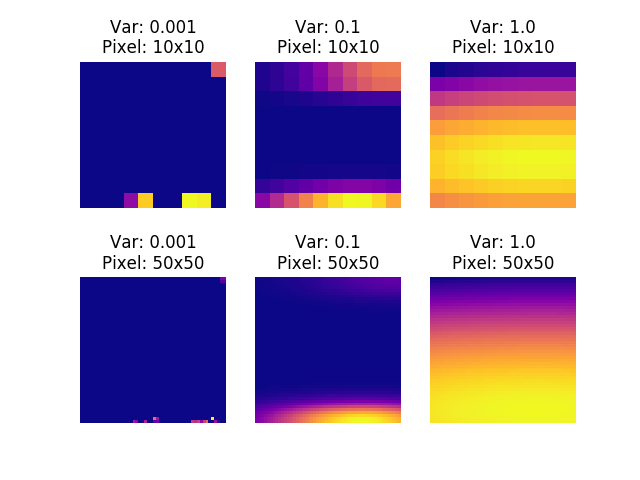
\includegraphics[width=0.9\textwidth]{images/comparacao_pis.png}
    \caption{Seis imagens de persistência do diagrama de dimensão $1$ da \autoref{fig:persdcircle}.} 
    \label{fig:persimgcircle}
    \fautor
\end{figure}

Observe a diferença entre os tamanhos escolhidos para as imagens. Com um tamanho maior, a informação fica mais fina,
porém a imagem fica esparsa. Além disso, com uma variância mais baixa os pontos ficam mais concentrados, enquanto
para valores mais altos há uma troca contínua entre as regiões dos pontos com maior frequência.

Todo o código para gerar o círculo com ruído, calcular os diagramas e imagens se encontram no 
\textit{Jupyter Notebook} no repositório da dissertação: \url{https://github.com/chronchi/dissertacao} na pasta
\textit{jupyter\_notebook}.

\section{Mapper}

Mapper é um algoritmo para visualização de dados com alta dimensão em $\mathbb{R}$ ou $\mathbb{R}^2$
através do uso de grafos e complexos simpliciais~\cite{mapper}. Ele é aplicado em diversas áreas,
sendo que uma delas é na inferência de formatos~\cite{Lum2013}. Nas próximas subseções iremos apresentar
a motivação topológica para o desenvolvimento do algoritmo assim como sua versão estatística, usada
em implementações. 

\subsection{Mapper topológico}

Seja $X$ um espaço topológico, $Z$ um espaço de parâmetros tais que $f \colon X \to Z$ é uma
função contínua. A função $f$ é chamada de filtro. Considere agora uma cobertura aberta
de $Z$, $\Set{U_\alpha}_{\alpha \in A}$ para algum conjunto finito de índices $A$. Como
$f$ é contínua, os conjuntos $f^{-1}(U_\alpha)$ também são abertos, portanto, temos uma
cobertura finita de $X$ dada por $\Set{f^{-1}(U_\alpha)}_{\alpha  \in A}$. 

Para cada um desses conjuntos abertos, considere suas respectivas componentes
conexas por caminho. Dessa forma podemos quebrar a cobertura em conjuntos $V(\alpha, i)$, 
em que $U_\alpha = \cup_i V(\alpha,i)$ e cada conjunto $V$ é aberto. Denote esta nova
cobertura por $\overline{\mathcal{U}}$.

Dada tal cobertura, podemos associar um complexo simplicial. Para uma cobertura $\mathcal{U}$
qualquer com um conjunto de índices finitos $A$, defina o nervo $N(\mathcal{U})$ como o 
complexo simplicial cujo conjunto de índices é $A$ e $\Set{\alpha_0, \dots, \alpha_k} \subset A$ 
gera um $k$-simplexo em $N(\mathcal{U})$ se, e somente se, $U_{\alpha_0} \cap \dots \cap U_{\alpha_k}$
é não-vazio. O Exemplo~\ref{ex:topmap} é um caso do mapper topológico.

\begin{ex}\label{ex:topmap}
    Seja $X$ um círculo únitario no plano e $Z=[-1,1]$. defina a função filtro como
    a projeção no eixo $y$, $f(x,y) = y$. Seja $\mathcal{U}$ a cobertura $\Set{[-1,-\frac{1}{3}), 
    (-\frac{1}{2},\frac{1}{2}), (\frac{1}{3}, 1]}$. Observe que $f^{-1}([-1,-\frac{1}{3}))$
    e $f^{-1}((\frac{1}{3}, 1])$  consistem de uma componente conexa cada, enquanto 
    $f^{-1}((-\frac{1}{2}, \frac{1}{2}))$ de duas componentes conexas. O complexo simplicial pode
    ser realizada como mostra a Figura~\ref{fig:topmap}
    \begin{figure}
        \centering
        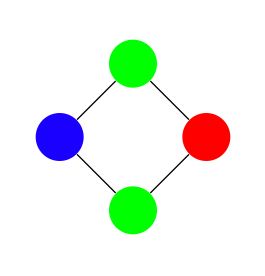
\includegraphics[width=0.7\textwidth]{images/topmap.png}
        \caption{Complexo simplicial associado a $X$, $Z$ e $f$ 
                 do Exemplo~\ref{ex:topmap}}
        \label{fig:topmap}
        \fautor
    \end{figure}
\end{ex}

\subsection{Mapper Estatístico} 

Vamos descrever agora a versão estatística do Mapper. Seja $X$ uma nuvem de pontos com $N$ pontos
e suponha que temos uma função $f \colon X \to \mathbb{R}$ cujos valores sabemos para cada ponto
em $X$. A função $f$ é chamada de filtro como anteriormente. Assuma também que podemos calcular a 
distância entre pontos de $X$. 

O primeiro passo é achar um intervalo ($I \subset \mathbb{R}$) da função $f$ sobre o conjunto
$X$ e uma cobertura dos dados sobre $I$. Após a seleção do intervalo $I$, temos mais dois parâmetros 
para determinar: as regiões menoras que dividirão $I$ e a porcentagem de interseção entre elas. 

Dados o intervalo $I$, cobertura $S$ de $I$ e $p$ a porcentagem de intereseção, tome um
intervalo $I_j \in S$ e considere os conjuntos $X_j = \Set{x \in X | f(x) \in I_j}$.
Logo, temos uma cobertura natural de $X \subset \cup X_j$. Esse passo é diferente da 
versão topológica, já que nós trabalhamos sobre um conjunto finito, temos que agrupar os pontos
em cada $X_j$, caso contrário dependemos da topologia, onde cada ponto seria uma componente conexa
e não teriamos nenhuma informação relevante. 

Portanto, devemos selecionar um algoritmo de agrupamento (Clustering), explicando o 
porque de precisar uma função distâcia entre os pontos. Então, para cada conjunto $X_j$ aplicamos 
o algoritmo de agrupamento e denotamos os clusters por $X_{ji}$. Observe que temos uma cobertura
de $X_j$ dessa forma. Na versão topológica, cada componente conexa por caminhos era tratada como
um vértice em um grafo, enquanto que não versão estatística cada cluster será tratado como
um vértice. Além disso, desenhamos uma aresta entre dois vértices (clusters) $X_{jk}$ e 
$X_{lm}$ toda vez que $X_{jk} \cap X_{lm} \neq \emptyset$.

\begin{ex}
    Este é um exemplo do mapper sendo aplicado em um círculo com ruídos. A função filtro
    é $f(x) = || x - p ||_2$, em que $p$ é o ponto mais a esquerda, em relação ao eixo $y$
    dos dados. As cores de cada vértice na Figure~ref{fig:statmap} correspondem à média
    do valor da função filtro em cada vértice, em que azul representa um valor baixo e 
    vermelho um valor alto. 

    O intervalo do filtro é $[0,4.2]$. O intervalo foi divido em $5$ partes menores com uma
    interseção de $20\%$. O algoritmo de agrupamento utilizado foi o \textit{single-linkage
    clustering}. Este exemplo foi retirado de~\cite{mapper}. 
    \begin{figure}
        \centering
        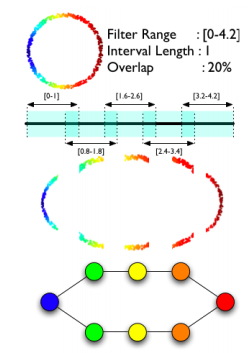
\includegraphics[width=0.7\textwidth]{images/statmap.png}
        \caption{Exemplo do Mapper sendo aplicado em um círculo com ruído.}
        \label{fig:statmap}
        \fautor
    \end{figure}
\end{ex} 

É possível também extender esta versão do algoritmo para uma com o espaço de parâmetros de dimensão
mais alta, com o $\mathbb{R}^2$, mais detalhes desta versão podem ser encontrados em~\cite{mapper}.

\subsection{Funções filtro}

A função filtro aplicada no algoritmo Mapper precisada ser escolhida com muito cuidado, pois o
grafo resultante depende da função escolhida. A seguir mostramos alguns exemplos para funções
filtro que capturam algumas propriedades dos conjuntos de dados.

\subsubsection{Ecentricidade}

Essa é uma família de função que capturam informações geométricas do conjunto de dados. Estas funções
identificam pontos longe do centro, sem especificar exatamente que ponto é o centro e onde ele está. 

Seja agora $p$ com $q \leq p < \infty$, então

\begin{equation}
    E_p(x) = \left( \frac{\sum_{y\in X} d(x,y)^p}{N} \right)^{\frac{1}{p}},
\end{equation}
and for $p = \infty$, set $E_\infty(x) = \max_{x' \in X} d(x,x')$. 

\subsubsection{Densidade} 

Seja $\epsilon > 0$. Então, $f_\epsilon$ é a estimativa do kernel gaussiano  
\begin{equation}
    f_\epsilon (x) = C_\epsilon \sum_y \exp\left( \frac{-d(x,y)^2}{\epsilon}\right),
\end{equation}
em que $x,y \in X$ e $C_\epsilon$ é uma constante tal que $\int f_\epsilon = 1$. A ideia 
do kernel gaussiano é que ele suaviza o conjunto de dados de forma que o parâmetro $\epsilon$ 
controla a suavidade. 

Podemos também usar funções que dependem do problema a ser trabalhado. Por exemplo, considere
um conjunto de proteínas com um score de estabilidade ou energia total associado a elas. Podemos
definir $f$ em cada proteína como os valores mencionados, pois esses já carregam informações
biológicas do conjunto. 

\subsection{Implementação} 

Uma variação da implementação do mapper pode ser encontrada em \url{https://github.com/chronchi/MapperMDS.jl}
desenvolvida pelo estudante. O algoritmo aceita uma matriz de distância como entrada e agrupa os pontos
utilizando DBScan \cite{Ester96} por padrão, mas aceita o algoritmo de agrupamento single linkage. 
Se este último for usado, recomenda-se usar o método da silhueta \cite{Rousseeuw1987} para escolher 
o melhor número de cluster em cada passo de agrupamento. 
